\chapter{\texttt{nimCSO} Basic Tutorial on Selecting Elements for High Entropy Alloy Modeling} \label{chap:nimcsotutorial}

The purpose of this guide is to demonstrate some common use cases of
\texttt{nimCSO} and go in a bit more into the details
of how it could be used, but it is not by any means extensive. If
something is not covered but you would like to see it here, please do
not hesitate to open an issue on GitHub and let use know!

\hypertarget{dataset-config-and-compilation}{%
\section{Dataset, Config, and
Compilation}\label{nimcsotutorial:dataset-config-and-compilation}}

To get started, let's first recap what we need to do to get
\texttt{nimCSO} up and running.

\textbf{1.} Install \texttt{nim} and dependencies, but \textbf{that's already
done for you if you are in the Codespace}. You can see what was run to
get the environment set up in the
\href{../.devcontainer/Dockerfile}{\texttt{Dockerfile}}.

\textbf{2.} Create the dataset. For now, let's just use the default one
(based on ULTERA Database) that comes with the package. Relative to this
notebook, the dataset is located at
\texttt{../dataList.txt}. Let's have a look at the
first few lines of the file to see what it looks like.

\begin{minted}[xleftmargin=3\parindent, linenos=true, fontsize=\small]{shell}
!head -n 8 ../dataList.txt
\end{minted}

\begin{minted}[xleftmargin=3\parindent, fontsize=\small, bgcolor=subtlegray]{output}
Al,Co,Cr,Cu,Fe,Ni
Nb,Ta,Ti
Co,Cr,Ni
Al,Co,Cr,Fe,Mn,Ni
Al,Co,Fe,Mo,Ni
Hf,Nb,Ti,V
Co,Cr,Fe,Nb,Ni
Al,Co,Cr,Cu,Fe,Ni
\end{minted}

\textbf{3.} Now, we need to create task
\texttt{config.yaml} file that will describe what we
are doing and point to our data file. That was already done for you in
the \href{config.yaml}{\texttt{config.yaml}} file, but
you are more than welcome to play and modify it.

\textbf{4.} Finally, we can run the \texttt{nimCSO}
package to get the results. To do so, we will use one long command you
can see below. Let's break it down:

\begin{itemize}
\item
  \texttt{nim} is the official Nim language compiler.
\item
  \texttt{c} instructs \texttt{nim}
  compiler to use \texttt{C} compiler to optimize and
  compile intermediate code. You can also use
  \texttt{cpp} to use \texttt{C++}
  compiler or \texttt{objc} to use
  \texttt{Objective-C} compiler. If you want, you can
  also compile directly with LLVM using
  \href{https://github.com/arnetheduck/nlvm}{\texttt{nlvm}},
  but it isn't pre-installed for you here.
\item
  \texttt{-f} is a flag to force the compiler to
  compile everything, even if the code didn't change. We want this
  because \texttt{config.yaml}, which tells
  \texttt{nimCSO} how to write itself, is not tracked
  by the compiler, but is critical to the compilation process (see two
  point below).
\item
  \texttt{-d:release} is a flag that tells the compiler
  to optimize the code for release. You can also use
  \texttt{-d:debug} to compile the code with better
  debugging support, but it will be slower and it will not prevent bugs
  from happening. There is also \texttt{-d:danger} that
  will disable all runtime checks and run a bit faster, but you no
  longer get memory safety guarantees.
\item
  \texttt{-d:configPath=config.yaml} is a flag pointing
  to \textbf{\texttt{config.yaml} that is read and
  tells \texttt{nimCSO} (not the compiler!) how to
  write itself \emph{before} the compilation starts.} That's the magic
  metaprogramming sauce enabling us to write functions which
  \texttt{C}/\texttt{C++} compiler can
  then turn into single deterministically allocated and exectuted
  machine code through
  \href{https://en.wikipedia.org/wiki/Inline_expansion}{inlining}.
\item
  \texttt{out:nimcso} is just telling the compiler to
  output the compiled binary right here and name it
  \texttt{nimcso}. You can name it whatever you want,
  but it's a good idea to name it something that makes sense.
\item
  \texttt{../src/nimcso} is pointing to the source code
  of \texttt{nimCSO} package to compile, relative to
  this notebook.
\end{itemize}

Let's run the command and see what happens! Shouldn't take more than a
few seconds.

\begin{minted}[xleftmargin=3\parindent, linenos=true, fontsize=\small]{shell}
nim c -f -d:release -d:configPath=config.yaml --out:nimcso ../src/nimcso 
\end{minted}

\begin{minted}[xleftmargin=3\parindent, fontsize=\small, bgcolor=subtlegray]{output}
...
config.yaml
CC: ../../../opt/conda/nim/lib/system/exceptions.nim
CC: ../../../opt/conda/nim/lib/std/private/digitsutils.nim
CC: ../../../opt/conda/nim/lib/std/assertions.nim
...
CC: nimcso/bitArrayAutoconfigured.nim
CC: nimcso.nim
Hint: orc; threads: on; opt: speed; options: -d:release
87026 lines; 7.635s; 257.383MiB peakmem; proj: /workspaces/nimCSO/src/nimcso; 
out: /workspaces/nimCSO/examples/nimcso[SuccessX]
\end{minted}

Now, let's run \texttt{nimCSO} and see what happens!

\begin{minted}[xleftmargin=3\parindent, linenos=true, fontsize=\small]{shell}
./nimcso
\end{minted}

\begin{figure}[H]
  \centering
  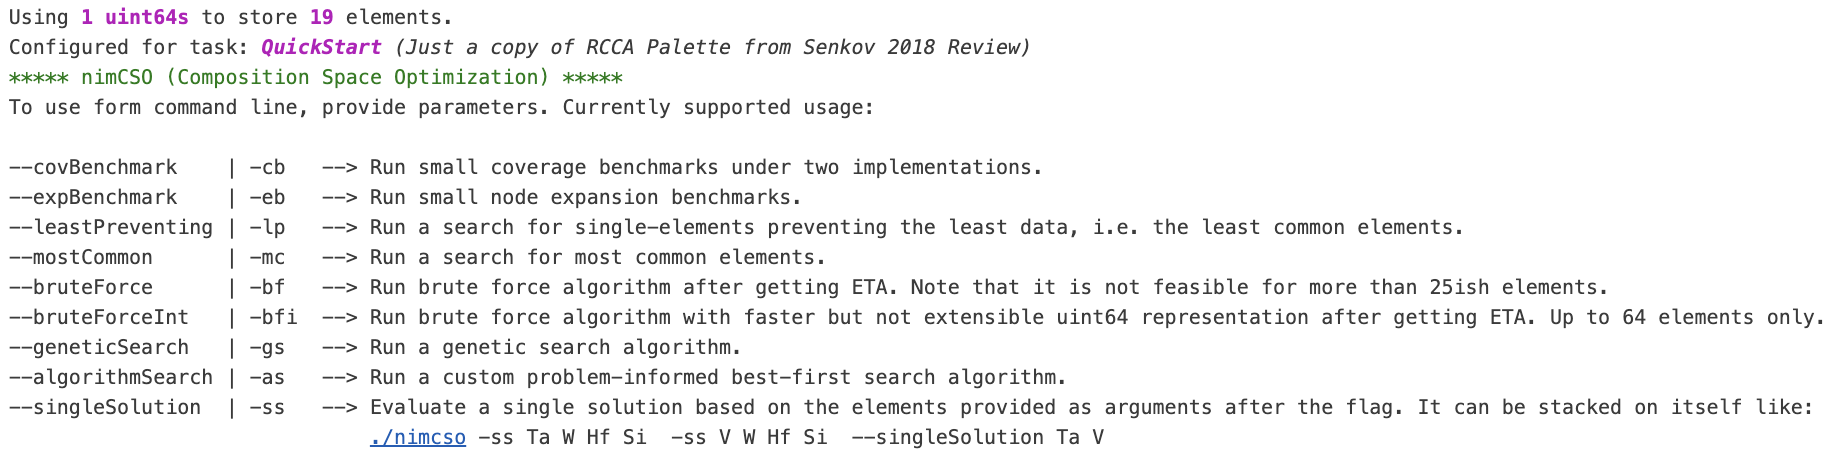
\includegraphics[width=0.97\textwidth]{nimcsotutorial/1.png}
\end{figure}

You should have seen a neat \texttt{help} message that
tells you how to use \texttt{nimCSO}. Let's start with
a ``coverage'' benchmark to see how fast can we check how many
datapoints will be removed from the dataset if we remove the first 5
elements of \texttt{elementOrder}.

\begin{minted}[xleftmargin=3\parindent, linenos=true, fontsize=\small]{shell}
./nimcso -cb
\end{minted}

\begin{figure}[H]
  \centering
  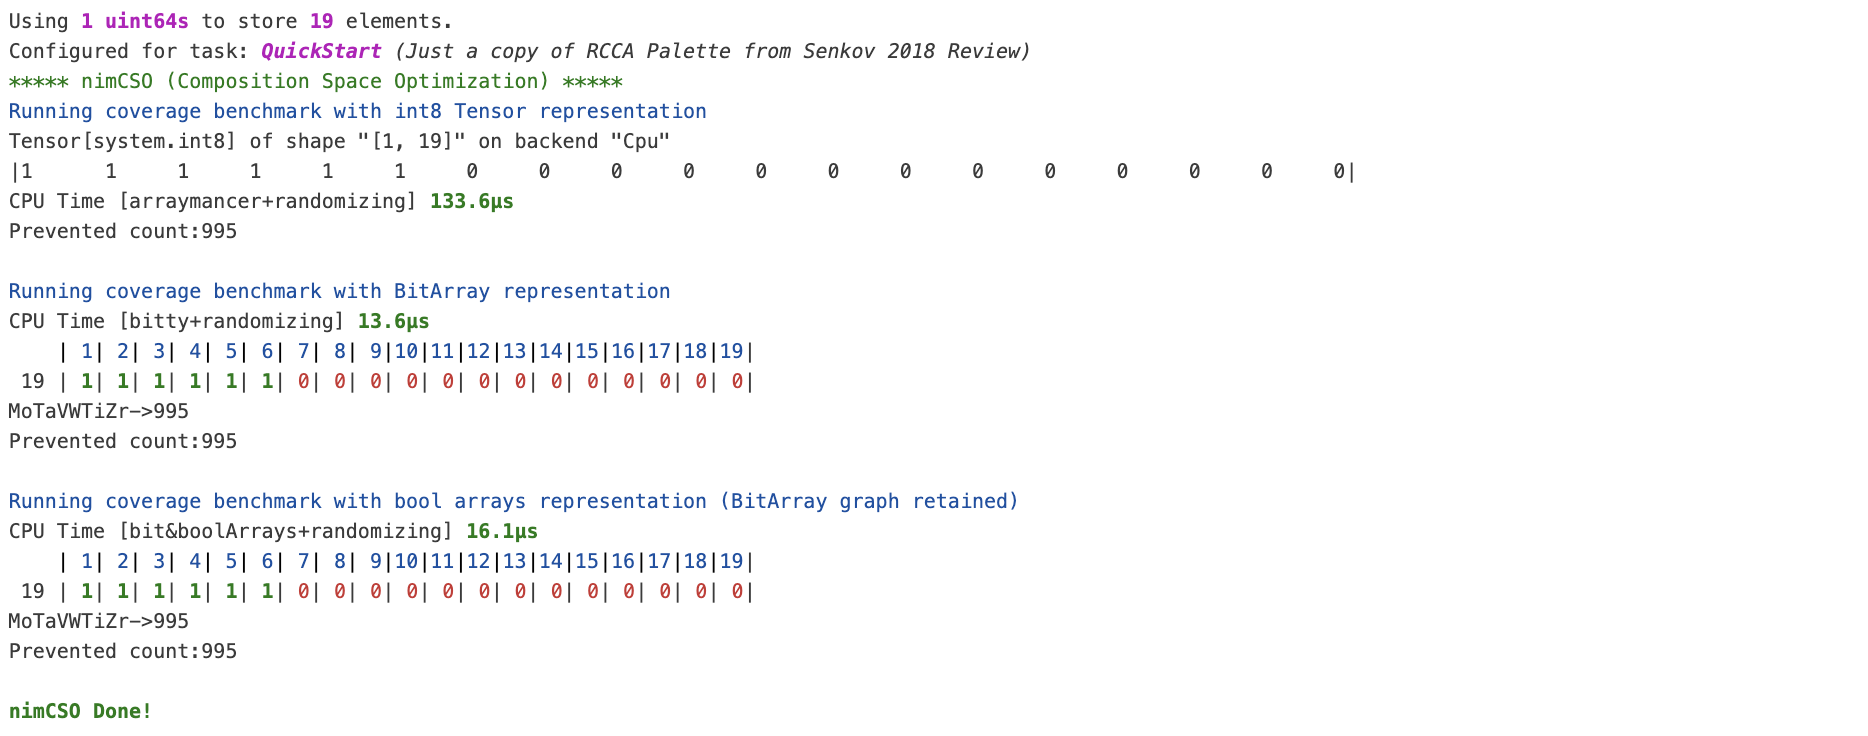
\includegraphics[width=0.97\textwidth]{nimcsotutorial/2.png}
\end{figure}

\hypertarget{key-routines-and-brute-forcing}{
\section{Key Routines and Brute Forcing}\label{nimcsotutorial:key-routines-and-brute-forcing}}

And if you were able to run that, you are all set to start using
\texttt{nimCSO}!

Let's try the simplest routine \texttt{mostCommon} or
\emph{What are the most common elements in the dataset?}

\begin{minted}[xleftmargin=3\parindent, linenos=true, fontsize=\small]{shell}
./nimcso --mostCommon
\end{minted}

\begin{figure}[H]
  \centering
  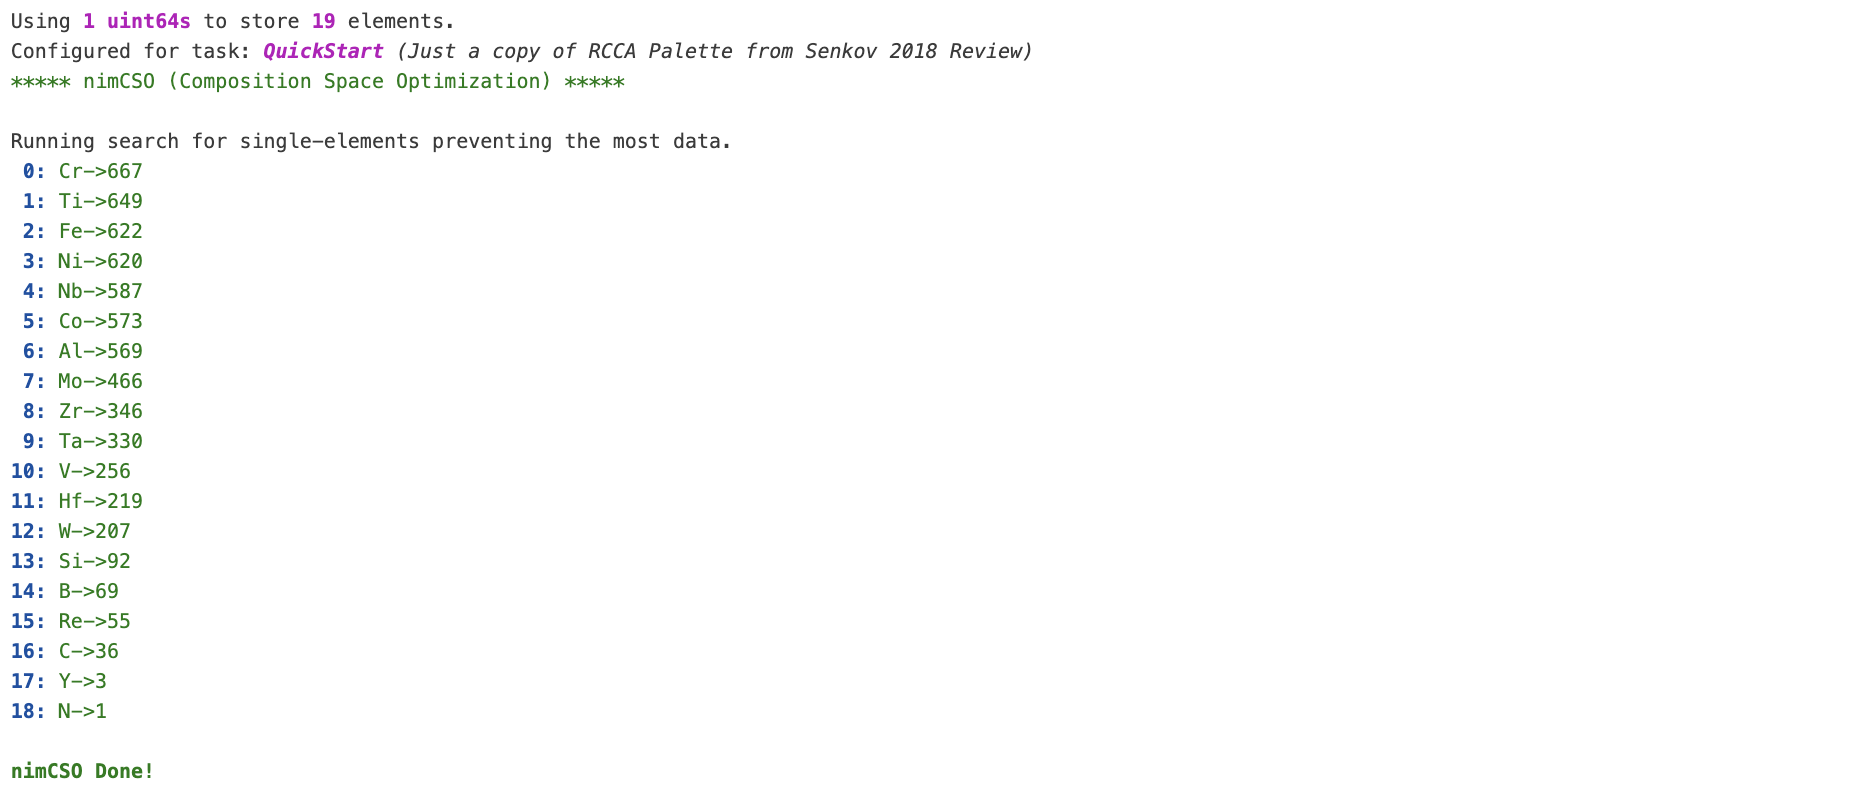
\includegraphics[width=0.97\textwidth]{nimcsotutorial/3.png}
\end{figure}

If you didn't modify anything, you should now see that elements like
\texttt{N}, \texttt{Y},
\texttt{C}, and \texttt{Re}, are not
very common in the dataset, while \texttt{Cr},
\texttt{Ti}, \texttt{Fe}, and
\texttt{Ni} are very common. When it comes to them, its
pretty obvious that removing the first group will be the first choice,
while the latter will be the last, if we want to keep the dataset as
extensive as possible.

The critical question here is, \emph{which of the intermediate elements
like \texttt{Hf}, \texttt{V},
\texttt{Ta}, or \texttt{Zr} should we
remove first?}

With a dataset spanning 19 elements, the solution space is around 0.5M,
so we can actually just brute force it in seconds :)

\begin{minted}[xleftmargin=3\parindent, linenos=true, fontsize=\small]{shell}
./nimcso -bfi
\end{minted}

\begin{figure}[H]
  \centering
  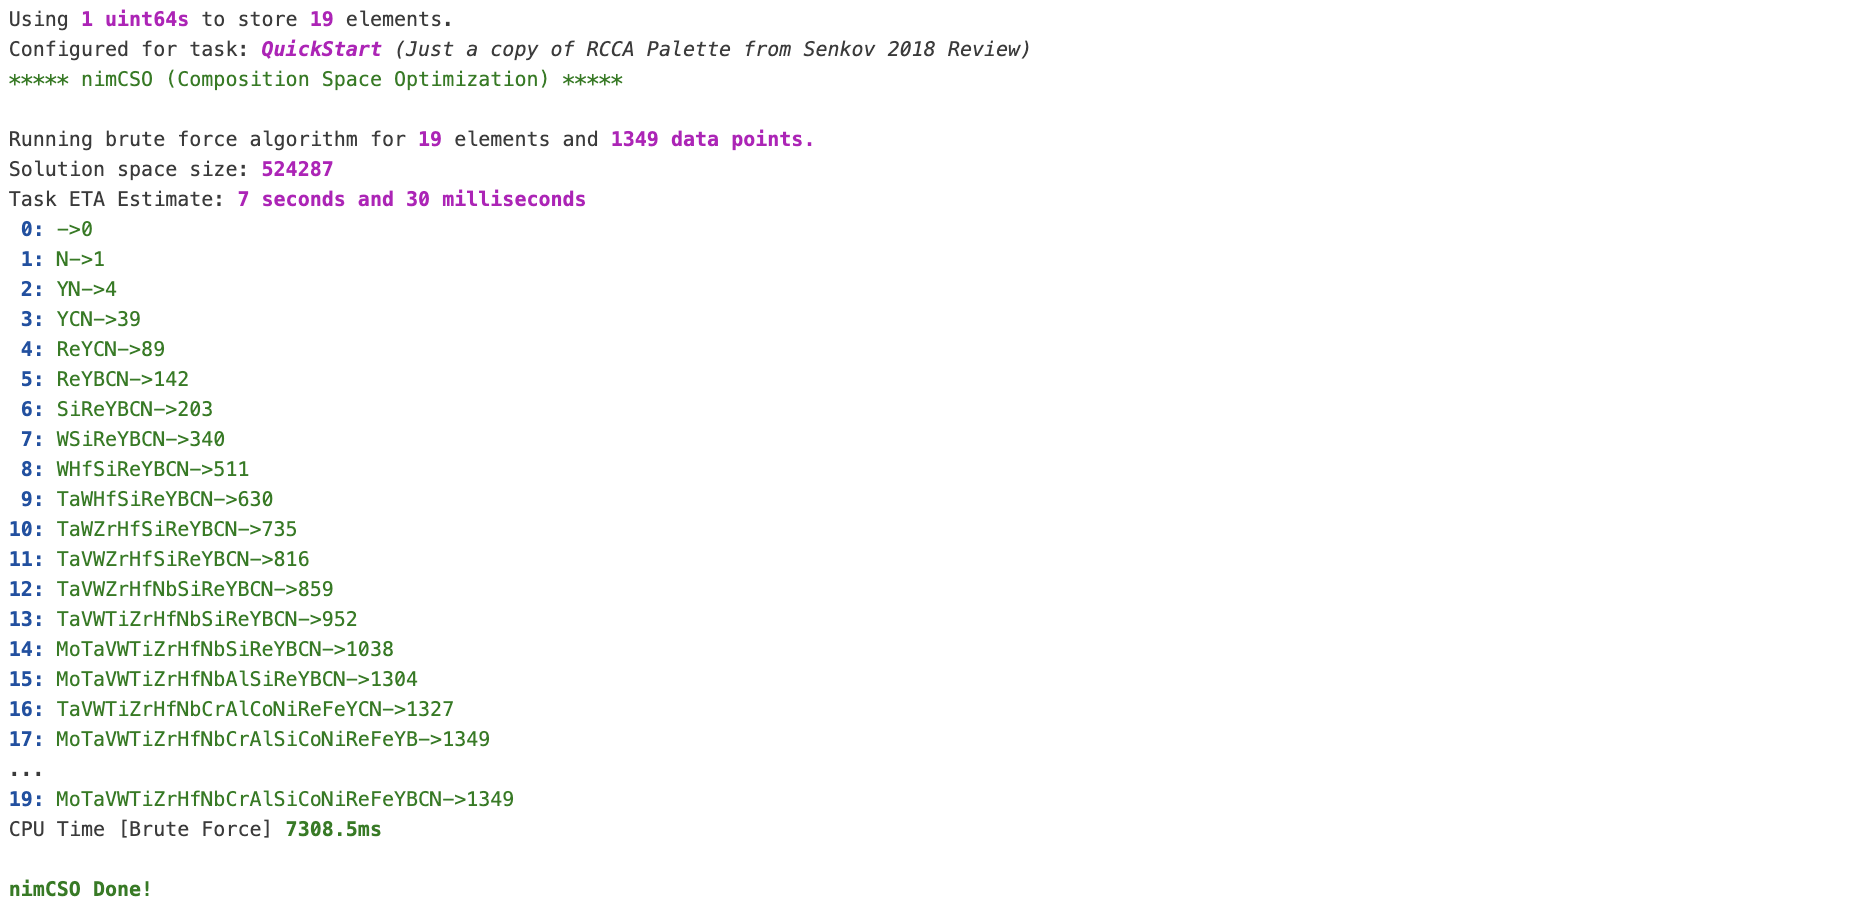
\includegraphics[width=0.97\textwidth]{nimcsotutorial/4.png}
\end{figure}

Let's look at the result! As expected, \texttt{N},
\texttt{Y}, \texttt{C}, and
\texttt{Re} are removed first (0-4) and then the trend
follows for a bit to \texttt{Hf} \textbf{The first
break is \texttt{V}, you can notice that it's better to
remove either or both \texttt{Ta} or
\texttt{Zr} first, despite the fact that they are
nearly 50\% more common than \texttt{V}} That's
because they often coocur with \texttt{Re} and
\texttt{Hf}, which are not common.

We can test exactly how much more data we will have if we remove
\texttt{Ta} insead of \texttt{V} by
using the \texttt{--singleSolution} /
\texttt{-ss} routine.

\begin{minted}[xleftmargin=3\parindent, linenos=true, fontsize=\small]{shell}
./nimcso -ss Ta W Hf Si Re Y B C N -ss V W Hf Si Re Y B C N
\end{minted}

\begin{figure}[H]
  \centering
  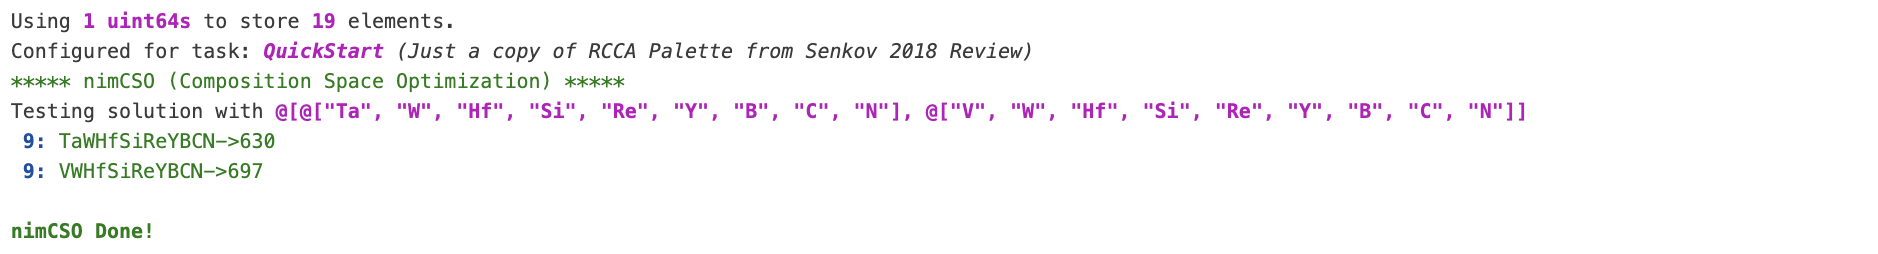
\includegraphics[width=0.97\textwidth]{nimcsotutorial/5.png}
\end{figure}

Wow! Looking at the \texttt{--mostCommon} output from
earlier, we can see that \textbf{\texttt{Ta} is present
in 74 more datapoints than \texttt{V}, but after
removing \texttt{WHfSiReYBCN}, picking
\texttt{V} as one of 10 elements to model will result
in 67 \emph{more} datapoints.} Relative to a dataset without
interdependencies, that's a 141 datapoint difference!

And another case that breaks from the ordering is
\texttt{Mo}, which is better to keep than much more
common \texttt{Nb}, and after
\texttt{Nb} is removed, even better thank keeping the
\texttt{Ti}, which is the second most common element in
the dataset!

Similarly to what we did with \texttt{V}
vs.~\texttt{Ta}, we can test how much more data we will
have if we remove \texttt{Nb} instead of
\texttt{Mo} by using the
\texttt{--singleSolution} /
\texttt{-ss} routine.

\begin{minted}[xleftmargin=3\parindent, linenos=true, fontsize=\small, breaklines]{shell}
./nimcso -ss Ta V W Zr Hf Nb Si Re Y B C N -ss Ta V W Zr Hf Mo Si Re Y B C N -ss Ta V W Zr Hf Ti Si Re Y B C N
\end{minted}

\begin{figure}[H]
  \centering
  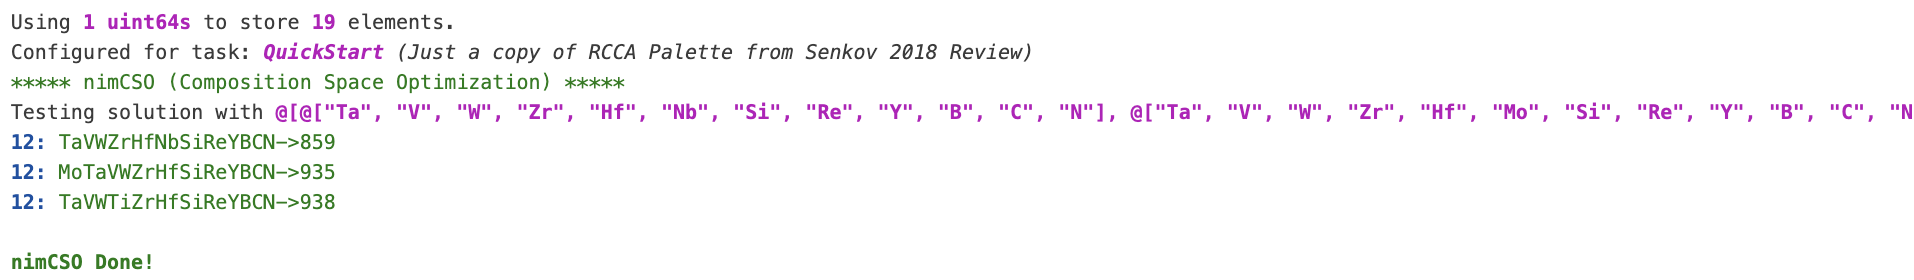
\includegraphics[width=0.97\textwidth]{nimcsotutorial/6.png}
\end{figure}

We can see that \textbf{\texttt{Nb} is present in 121
more datapoints than \texttt{Mo}, but after removing
\texttt{TaVWZrHfSiReYBCN}, picking
\texttt{Mo} as one of 7 elements to model will result
in 76 \emph{more} datapoints.} Relative to a dataset without
interdependencies, that's a 197 datapoint difference, which is even more
than the \texttt{Ta} vs.~\texttt{V}
case! Additionally, we can see that \texttt{Ti} is only
3 datapoints better than \texttt{Mo}, despite being
present in 183 more datapoints than \texttt{Mo}.

\hypertarget{algorithm-search}{%
\section{Algorithm Search}\label{nimcsotutorial:algorithm-search}}

The
\texttt{--bruteForceInt}/\texttt{-bfi}
routine we used to find the solutions worked great for our 19-element
dataset and took only a few seconds on the low-performance Codespace
machine, but in many cases dimensionality of the problem will be too
high to brute force it.

Let's now try to use the
\texttt{--algorithmSearch}/\texttt{-as}
routine, which takes advantage of some assumptions known to be valid or
likely to be valid (see manuscript), to limit the search space and find
the solution in a reasonable time. Let's try it now!

\begin{minted}[xleftmargin=3\parindent, linenos=true, fontsize=\small]{shell}
./nimcso -as
\end{minted}

\begin{figure}[H]
  \centering
  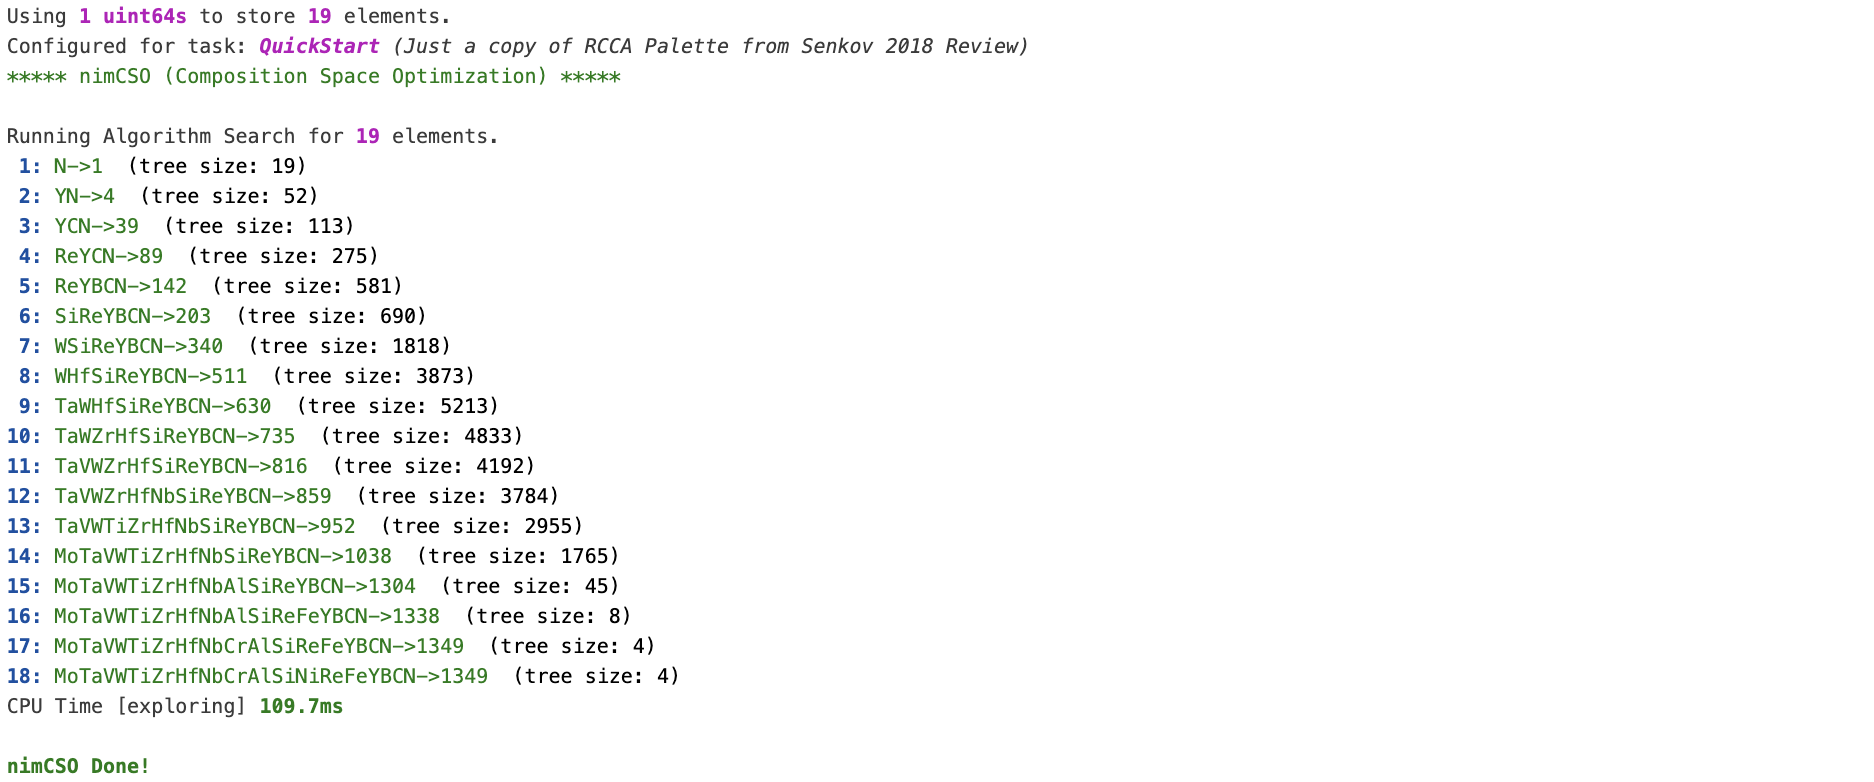
\includegraphics[width=0.97\textwidth]{nimcsotutorial/7.png}
\end{figure}

As you can see, \textbf{the algorithm reproduced the same results as the
brute force search around 100 times faster}, except for third-to-last
step because dataset had points with at least 3 elements breaking its
backtracking assumptions.

\hypertarget{genetic-search}{%
\section{Genetic Search}\label{nimcsotutorial:genetic-search}}

For cases where the dimensionality of the problem is too high to either
brute-force or use the algorithm search, we can still use the
\texttt{--geneticSearch}/\texttt{-gs}
routine to find the solution in a reasonable time. Let's try it now!

Please note that the results are stochastic, so you might get different
results than ones shown below if you run the command again.

\begin{minted}[xleftmargin=3\parindent, linenos=true, fontsize=\small]{shell}
./nimcso -gs
\end{minted}

\begin{figure}[H]
  \centering
  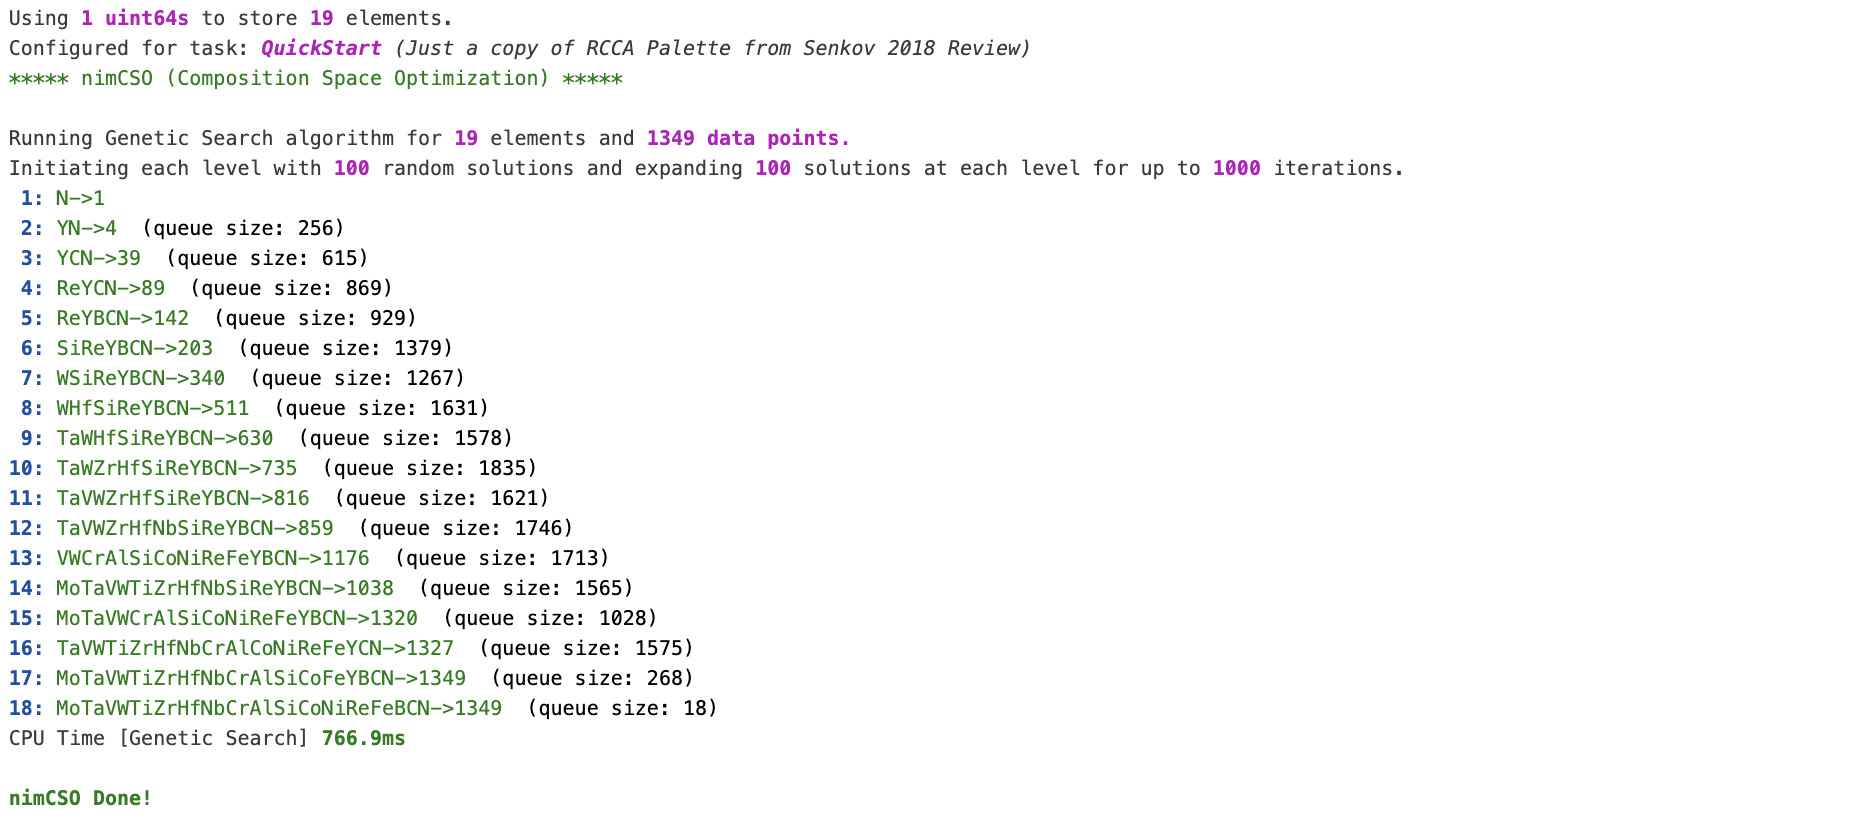
\includegraphics[width=0.97\textwidth]{nimcsotutorial/8.png}
\end{figure}

\hypertarget{summary}{%
\subsection{Summary}\label{nimcsotutorial:summary}}

Now, you should be able to apply \texttt{nimCSO} to
your own dataset and get some valuable insights on how to model it!

If you are working in a Codespace, you can just do everything right in
this notebook by simply modifying the
\texttt{config.yaml} file and running the commands you
just learned about. The Codespace will be persisted until you explicitly
delete it, so you can come back to it later and continue your work by
clicking on the link in the ``Open in Codespaces'' badge in the README
of the repository and resuming your work.
